\begin{figure}[h!]
\setlength{\unitlength}{\textwidth}

  \begin{picture}(0.95,0.5)(0,0.8)
   
  \put(0.2,0.76){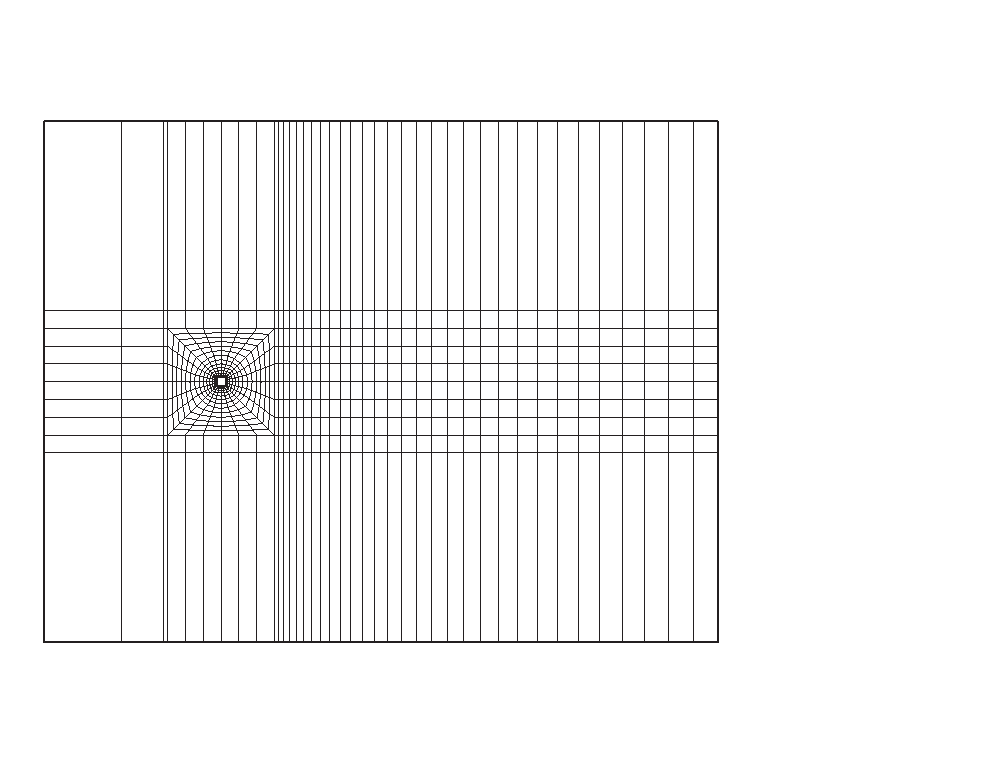
\includegraphics[width=0.8\unitlength]{./chapter-methodology/fnp/square-mesh.eps}}         
      
      
   

      	

  \end{picture}

 \caption{Macro element arrangement of the domain of the square cross section. The inlet extending  $20D$ towards upstream from the centre of the body, while the outlet extended $60D$ downstream from the centre of the body. The lateral boundaries were placed $20D$ away from the centre of the body}
    \label{fig:square-mesh}
\end{figure}